\chapter{Sammenhængende grafer}
Veje i en graf viser hvilke ruter der er rundt i en graf. Dette er relevant for at finde ruter til en GPS, et computernetværk eller andet hvor der er behov for at bestemme en rute gennem flere steder. 

\section{Veje}
En vej i en graf defineres i Definition \ref{def_vej}.

\begin{defn}
\label{def_vej}
Lad $n \in  \mathbb{Z}^{+}$ og lad $G$ være en ikke-orienteret graf. 
En \textit{vej} af \textit{længde} $n$ fra $u$ til $v$ i $G$ er en sekvens af $n$ kanter $e_1, ..., e_n$ i $G$, for hvilke der eksisterer en sekvens $x_0=u,x_1,...,x_{n-1},x_n=v$ af punkter så $e_i$ har endepunkterne $x_{i-1}$ og $x_1$ for $i=1,...,n$.
\end{defn}

\noindent Når der er tale om en vej gennem en simpel graf, noteres denne som sekvensen af de punkter den går igennem $x_0, x_1,...,x_n$. 
I et særligt tilfælde, kan en vej kaldes en kreds efter definition \ref{def_kredse}.
En vej eller kreds er \textit{simpel} hvis den ikke indeholder den samme kant mere end én gang. 

\begin{exmp}
\label{ex_vej}
På den simple graf i Figur \ref{graf_vej} ses en simpel vej $A,B,E,F$ af længden 3, fordi vejen går gennem de tre kanter $\lbrace A,B \rbrace$, $\lbrace B,E \rbrace$ og $\lbrace E,F \rbrace$. 
Denne vej er simpel, fordi den ikke går gennem den samme kant mere end en gang. 
Derimod er $A,B,D,E$ ikke en vej, fordi $\lbrace B,D \rbrace$ ikke er en kant. 
Vejen $A,B,C,E,B,A$ er også en vej, men den er ikke simpel, fordi den går gennem kanten $\lbrace A,B \rbrace$ to gange. 

\end{exmp}

\begin{figure}[h]
\centering
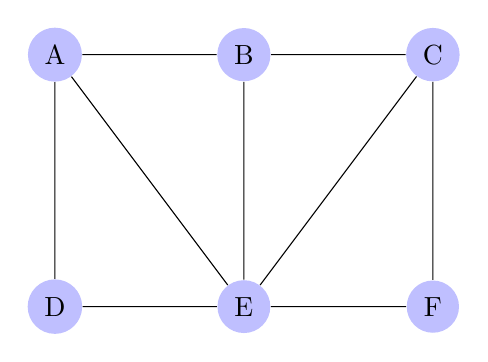
\begin{tikzpicture}
[scale=.8,auto=left,every node/.style={circle,fill=blue!25}]
  \node (n6) at (3,2) {D};
  \node (n4) at (3,6) {A};
  \node (n5) at (6,2) {E};
  \node (n1) at (6,6) {B};
  \node (n2) at (9,2) {F};
  \node (n3) at (9,6) {C};
  \foreach \from/\to in {n6/n4,n4/n5,n5/n1,n2/n5,n2/n3,n3/n1,n1/n4,n6/n5,n5/n3}
    \draw (\from) -- (\to);
\end{tikzpicture}
\caption{graf} 
\label{graf_vej}
\end{figure}

\begin{defn}
\label{def_kredse}
En vej er en \textit{kreds} hvis den begynder og ender i samme punkt, $u=v$ og $n>0$.
Vejen eller kredsen siges at gå gennem punkterne $x_1,x_2,...,x_{n-1}$ eller passere gennem kanterne $e_1, e_2,...e_n$.
\end{defn}

\begin{exmp}
I Figur \ref{graf_kreds} ses en kreds, $A,B,C,E,D,A$, som har længden 5, fordi den går gennem 5 kanter. Det er en kreds fordi den begynder og ender i punktet $A$
\end{exmp}

\begin{figure}[h]
\centering
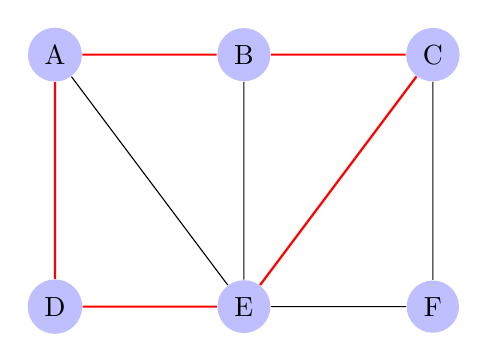
\begin{tikzpicture}
[scale=.8,auto=left,every node/.style={circle,fill=blue!25}]
  \node (n6) at (3,2) {D};
  \node (n4) at (3,6) {A};
  \node (n5) at (6,2) {E};
  \node (n1) at (6,6) {B};
  \node (n2) at (9,2) {F};
  \node (n3) at (9,6) {C};
  \draw (n6) edge [red, thick] (n4);
  \draw (n6) edge [red, thick] (n5);
  \draw (n5) edge [red, thick] (n3);
  \draw (n3) edge [red, thick] (n1);
  \draw (n1) edge [red, thick] (n4);
  \foreach \from/\to in {n5/n1,n2/n5,n2/n3,n4/n5}
    \draw (\from) -- (\to);
\end{tikzpicture}
\caption{Kreds} 
\label{graf_kreds}
\end{figure}